% ---------------------------------------------------------------
%  EnergyTech / معهد الطاقة  --  Chapter 04, version C
%  Questions + answer choices + QR codes.
%  Scale diagrams are TikZ; the two labelled instrument photographs
%  live in figures/.
%  Compile with pdflatex (needs the 'qrcode' package).
% ---------------------------------------------------------------
\documentclass[11pt]{article}
\usepackage[a4paper,margin=1.8cm]{geometry}
\usepackage{amsmath,amssymb}
\usepackage{enumitem}
\usepackage{qrcode}
\usepackage{graphicx}
\usepackage{xcolor}
\usepackage[hidelinks]{hyperref}
\usepackage{multicol}

\setlength{\parindent}{0pt}
\setlength{\columnsep}{20pt}
\graphicspath{{figures/}}

\newcommand{\incfig}[2]{%
  \par\smallskip\begingroup\centering
  \ifdim #1pt>\linewidth\relax
    \includegraphics[width=\linewidth]{#2}%
  \else
    \includegraphics[width=#1pt]{#2}%
  \fi
  \par\endgroup\smallskip}

\newenvironment{Qbox}[2]{%
  \par\medskip\noindent\begin{minipage}{\linewidth}%
  \hrule\medskip%
  \textbf{Q#1)}\hfill\textbf{\underline{#2}}\par\smallskip%
}{\par\end{minipage}\par\medskip}

\newlist{choices}{enumerate}{1}
\setlist[choices]{label=\Alph*), itemsep=1pt, topsep=3pt, parsep=0pt, leftmargin=2em}
% ---------------------------------------------------------------

% ================= figure styles =================
\usepackage{tikz}
\usetikzlibrary{arrows.meta,calc,shadings}

\definecolor{figline}{RGB}{30,30,30}
\definecolor{figpanel}{RGB}{243,243,243}
\definecolor{figmark}{RGB}{63,63,160}
\definecolor{figbody}{RGB}{232,234,238}
\definecolor{figthimble}{RGB}{205,210,219}

\tikzset{
  sc/.style   ={draw=figline, line width=0.5pt, line cap=butt},
  scb/.style  ={draw=figline, line width=0.8pt},
  lab/.style  ={font=\small\bfseries, inner sep=1pt},
  labs/.style ={font=\scriptsize\bfseries, inner sep=1pt},
  ptr/.style ={draw=figmark, line width=1pt, -{Latex[length=4pt,width=3.5pt]}},
}

\newcommand{\figbox}[1]{%
  \par\smallskip\begingroup\centering
  \sbox0{#1}%
  \ifdim\wd0>\linewidth \resizebox{\linewidth}{!}{\usebox0}\else\usebox0\fi
  \par\endgroup\smallskip}

% ---- figure definitions ----
\newcommand{\figQBZ}{%
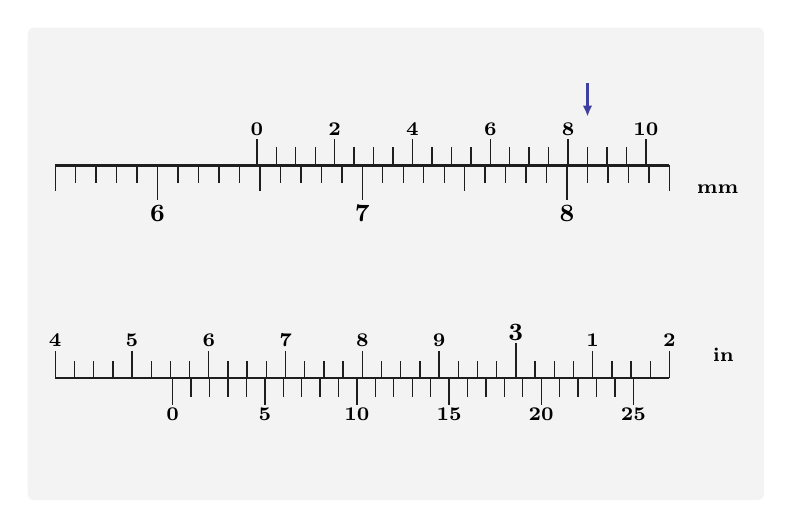
\begin{tikzpicture}[scale=1]
  \fill[figpanel,rounded corners=2pt] (-0.35,-1.55) rectangle (9,4.45);
  \begin{scope}[yshift=2.70cm]
  \draw[scb] (0,0) -- (7.8,0);
  \draw[sc] (0,0) -- (0,-0.32);
  \draw[sc] (0.26,0) -- (0.26,-0.22);
  \draw[sc] (0.52,0) -- (0.52,-0.22);
  \draw[sc] (0.78,0) -- (0.78,-0.22);
  \draw[sc] (1.04,0) -- (1.04,-0.22);
  \draw[sc] (1.3,0) -- (1.3,-0.44);
  \node[lab,below] at (1.3,-0.46) {6};
  \draw[sc] (1.56,0) -- (1.56,-0.22);
  \draw[sc] (1.82,0) -- (1.82,-0.22);
  \draw[sc] (2.08,0) -- (2.08,-0.22);
  \draw[sc] (2.34,0) -- (2.34,-0.22);
  \draw[sc] (2.6,0) -- (2.6,-0.32);
  \draw[sc] (2.86,0) -- (2.86,-0.22);
  \draw[sc] (3.12,0) -- (3.12,-0.22);
  \draw[sc] (3.38,0) -- (3.38,-0.22);
  \draw[sc] (3.64,0) -- (3.64,-0.22);
  \draw[sc] (3.9,0) -- (3.9,-0.44);
  \node[lab,below] at (3.9,-0.46) {7};
  \draw[sc] (4.16,0) -- (4.16,-0.22);
  \draw[sc] (4.42,0) -- (4.42,-0.22);
  \draw[sc] (4.68,0) -- (4.68,-0.22);
  \draw[sc] (4.94,0) -- (4.94,-0.22);
  \draw[sc] (5.2,0) -- (5.2,-0.32);
  \draw[sc] (5.46,0) -- (5.46,-0.22);
  \draw[sc] (5.72,0) -- (5.72,-0.22);
  \draw[sc] (5.98,0) -- (5.98,-0.22);
  \draw[sc] (6.24,0) -- (6.24,-0.22);
  \draw[sc] (6.5,0) -- (6.5,-0.44);
  \node[lab,below] at (6.5,-0.46) {8};
  \draw[sc] (6.76,0) -- (6.76,-0.22);
  \draw[sc] (7.02,0) -- (7.02,-0.22);
  \draw[sc] (7.28,0) -- (7.28,-0.22);
  \draw[sc] (7.54,0) -- (7.54,-0.22);
  \draw[sc] (7.8,0) -- (7.8,-0.32);
  \draw[sc] (2.561,0) -- (2.561,0.34);
  \node[labs,above] at (2.561,0.34) {0};
  \draw[sc] (2.808,0) -- (2.808,0.24);
  \draw[sc] (3.055,0) -- (3.055,0.24);
  \draw[sc] (3.302,0) -- (3.302,0.24);
  \draw[sc] (3.549,0) -- (3.549,0.34);
  \node[labs,above] at (3.549,0.34) {2};
  \draw[sc] (3.796,0) -- (3.796,0.24);
  \draw[sc] (4.043,0) -- (4.043,0.24);
  \draw[sc] (4.29,0) -- (4.29,0.24);
  \draw[sc] (4.537,0) -- (4.537,0.34);
  \node[labs,above] at (4.537,0.34) {4};
  \draw[sc] (4.784,0) -- (4.784,0.24);
  \draw[sc] (5.031,0) -- (5.031,0.24);
  \draw[sc] (5.278,0) -- (5.278,0.24);
  \draw[sc] (5.525,0) -- (5.525,0.34);
  \node[labs,above] at (5.525,0.34) {6};
  \draw[sc] (5.772,0) -- (5.772,0.24);
  \draw[sc] (6.019,0) -- (6.019,0.24);
  \draw[sc] (6.266,0) -- (6.266,0.24);
  \draw[sc] (6.513,0) -- (6.513,0.34);
  \node[labs,above] at (6.513,0.34) {8};
  \draw[sc] (6.76,0) -- (6.76,0.24);
  \draw[sc] (7.007,0) -- (7.007,0.24);
  \draw[sc] (7.254,0) -- (7.254,0.24);
  \draw[sc] (7.501,0) -- (7.501,0.34);
  \node[labs,above] at (7.501,0.34) {10};
  \draw[ptr] (6.76,1.05) -- (6.76,0.62);
  \node[labs,left] at (8.72,-0.30) {mm};
  \end{scope}
  \begin{scope}[yshift=0cm]
  \draw[scb] (0,0) -- (7.8,0);
  \draw[sc] (0,0) -- (0,0.34);
  \node[labs,above] at (0,0.36) {4};
  \draw[sc] (0.2438,0) -- (0.2438,0.22);
  \draw[sc] (0.4875,0) -- (0.4875,0.22);
  \draw[sc] (0.7313,0) -- (0.7313,0.22);
  \draw[sc] (0.975,0) -- (0.975,0.34);
  \node[labs,above] at (0.975,0.36) {5};
  \draw[sc] (1.2188,0) -- (1.2188,0.22);
  \draw[sc] (1.4625,0) -- (1.4625,0.22);
  \draw[sc] (1.7063,0) -- (1.7063,0.22);
  \draw[sc] (1.95,0) -- (1.95,0.34);
  \node[labs,above] at (1.95,0.36) {6};
  \draw[sc] (2.1938,0) -- (2.1938,0.22);
  \draw[sc] (2.4375,0) -- (2.4375,0.22);
  \draw[sc] (2.6813,0) -- (2.6813,0.22);
  \draw[sc] (2.925,0) -- (2.925,0.34);
  \node[labs,above] at (2.925,0.36) {7};
  \draw[sc] (3.1688,0) -- (3.1688,0.22);
  \draw[sc] (3.4125,0) -- (3.4125,0.22);
  \draw[sc] (3.6563,0) -- (3.6563,0.22);
  \draw[sc] (3.9,0) -- (3.9,0.34);
  \node[labs,above] at (3.9,0.36) {8};
  \draw[sc] (4.1438,0) -- (4.1438,0.22);
  \draw[sc] (4.3875,0) -- (4.3875,0.22);
  \draw[sc] (4.6313,0) -- (4.6313,0.22);
  \draw[sc] (4.875,0) -- (4.875,0.34);
  \node[labs,above] at (4.875,0.36) {9};
  \draw[sc] (5.1188,0) -- (5.1188,0.22);
  \draw[sc] (5.3625,0) -- (5.3625,0.22);
  \draw[sc] (5.6063,0) -- (5.6063,0.22);
  \draw[sc] (5.85,0) -- (5.85,0.44);
  \node[lab,above] at (5.85,0.44) {3};
  \draw[sc] (6.0938,0) -- (6.0938,0.22);
  \draw[sc] (6.3375,0) -- (6.3375,0.22);
  \draw[sc] (6.5813,0) -- (6.5813,0.22);
  \draw[sc] (6.825,0) -- (6.825,0.34);
  \node[labs,above] at (6.825,0.36) {1};
  \draw[sc] (7.0688,0) -- (7.0688,0.22);
  \draw[sc] (7.3125,0) -- (7.3125,0.22);
  \draw[sc] (7.5563,0) -- (7.5563,0.22);
  \draw[sc] (7.8,0) -- (7.8,0.34);
  \node[labs,above] at (7.8,0.36) {2};
  \draw[sc] (1.4918,0) -- (1.4918,-0.34);
  \node[labs,below] at (1.4918,-0.34) {0};
  \draw[sc] (1.7258,0) -- (1.7258,-0.24);
  \draw[sc] (1.9598,0) -- (1.9598,-0.24);
  \draw[sc] (2.1938,0) -- (2.1938,-0.24);
  \draw[sc] (2.4278,0) -- (2.4278,-0.24);
  \draw[sc] (2.6618,0) -- (2.6618,-0.34);
  \node[labs,below] at (2.6618,-0.34) {5};
  \draw[sc] (2.8958,0) -- (2.8958,-0.24);
  \draw[sc] (3.1298,0) -- (3.1298,-0.24);
  \draw[sc] (3.3638,0) -- (3.3638,-0.24);
  \draw[sc] (3.5978,0) -- (3.5978,-0.24);
  \draw[sc] (3.8318,0) -- (3.8318,-0.34);
  \node[labs,below] at (3.8318,-0.34) {10};
  \draw[sc] (4.0658,0) -- (4.0658,-0.24);
  \draw[sc] (4.2998,0) -- (4.2998,-0.24);
  \draw[sc] (4.5337,0) -- (4.5337,-0.24);
  \draw[sc] (4.7677,0) -- (4.7677,-0.24);
  \draw[sc] (5.0017,0) -- (5.0017,-0.34);
  \node[labs,below] at (5.0017,-0.34) {15};
  \draw[sc] (5.2357,0) -- (5.2357,-0.24);
  \draw[sc] (5.4697,0) -- (5.4697,-0.24);
  \draw[sc] (5.7037,0) -- (5.7037,-0.24);
  \draw[sc] (5.9377,0) -- (5.9377,-0.24);
  \draw[sc] (6.1718,0) -- (6.1718,-0.34);
  \node[labs,below] at (6.1718,-0.34) {20};
  \draw[sc] (6.4058,0) -- (6.4058,-0.24);
  \draw[sc] (6.6398,0) -- (6.6398,-0.24);
  \draw[sc] (6.8738,0) -- (6.8738,-0.24);
  \draw[sc] (7.1078,0) -- (7.1078,-0.24);
  \draw[sc] (7.3418,0) -- (7.3418,-0.34);
  \node[labs,below] at (7.3418,-0.34) {25};
  \node[labs,left] at (8.66,0.30) {in};
  \end{scope}
\end{tikzpicture}
}

\newcommand{\figQBA}{%
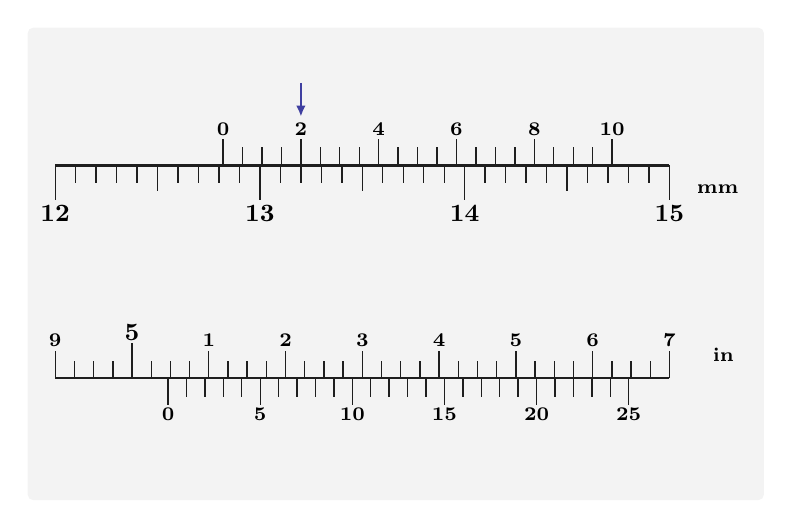
\begin{tikzpicture}[scale=1]
  \fill[figpanel,rounded corners=2pt] (-0.35,-1.55) rectangle (9,4.45);
  \begin{scope}[yshift=2.70cm]
  \draw[scb] (0,0) -- (7.8,0);
  \draw[sc] (0,0) -- (0,-0.44);
  \node[lab,below] at (0,-0.46) {12};
  \draw[sc] (0.26,0) -- (0.26,-0.22);
  \draw[sc] (0.52,0) -- (0.52,-0.22);
  \draw[sc] (0.78,0) -- (0.78,-0.22);
  \draw[sc] (1.04,0) -- (1.04,-0.22);
  \draw[sc] (1.3,0) -- (1.3,-0.32);
  \draw[sc] (1.56,0) -- (1.56,-0.22);
  \draw[sc] (1.82,0) -- (1.82,-0.22);
  \draw[sc] (2.08,0) -- (2.08,-0.22);
  \draw[sc] (2.34,0) -- (2.34,-0.22);
  \draw[sc] (2.6,0) -- (2.6,-0.44);
  \node[lab,below] at (2.6,-0.46) {13};
  \draw[sc] (2.86,0) -- (2.86,-0.22);
  \draw[sc] (3.12,0) -- (3.12,-0.22);
  \draw[sc] (3.38,0) -- (3.38,-0.22);
  \draw[sc] (3.64,0) -- (3.64,-0.22);
  \draw[sc] (3.9,0) -- (3.9,-0.32);
  \draw[sc] (4.16,0) -- (4.16,-0.22);
  \draw[sc] (4.42,0) -- (4.42,-0.22);
  \draw[sc] (4.68,0) -- (4.68,-0.22);
  \draw[sc] (4.94,0) -- (4.94,-0.22);
  \draw[sc] (5.2,0) -- (5.2,-0.44);
  \node[lab,below] at (5.2,-0.46) {14};
  \draw[sc] (5.46,0) -- (5.46,-0.22);
  \draw[sc] (5.72,0) -- (5.72,-0.22);
  \draw[sc] (5.98,0) -- (5.98,-0.22);
  \draw[sc] (6.24,0) -- (6.24,-0.22);
  \draw[sc] (6.5,0) -- (6.5,-0.32);
  \draw[sc] (6.76,0) -- (6.76,-0.22);
  \draw[sc] (7.02,0) -- (7.02,-0.22);
  \draw[sc] (7.28,0) -- (7.28,-0.22);
  \draw[sc] (7.54,0) -- (7.54,-0.22);
  \draw[sc] (7.8,0) -- (7.8,-0.44);
  \node[lab,below] at (7.8,-0.46) {15};
  \draw[sc] (2.132,0) -- (2.132,0.34);
  \node[labs,above] at (2.132,0.34) {0};
  \draw[sc] (2.379,0) -- (2.379,0.24);
  \draw[sc] (2.626,0) -- (2.626,0.24);
  \draw[sc] (2.873,0) -- (2.873,0.24);
  \draw[sc] (3.12,0) -- (3.12,0.34);
  \node[labs,above] at (3.12,0.34) {2};
  \draw[sc] (3.367,0) -- (3.367,0.24);
  \draw[sc] (3.614,0) -- (3.614,0.24);
  \draw[sc] (3.861,0) -- (3.861,0.24);
  \draw[sc] (4.108,0) -- (4.108,0.34);
  \node[labs,above] at (4.108,0.34) {4};
  \draw[sc] (4.355,0) -- (4.355,0.24);
  \draw[sc] (4.602,0) -- (4.602,0.24);
  \draw[sc] (4.849,0) -- (4.849,0.24);
  \draw[sc] (5.096,0) -- (5.096,0.34);
  \node[labs,above] at (5.096,0.34) {6};
  \draw[sc] (5.343,0) -- (5.343,0.24);
  \draw[sc] (5.59,0) -- (5.59,0.24);
  \draw[sc] (5.837,0) -- (5.837,0.24);
  \draw[sc] (6.084,0) -- (6.084,0.34);
  \node[labs,above] at (6.084,0.34) {8};
  \draw[sc] (6.331,0) -- (6.331,0.24);
  \draw[sc] (6.578,0) -- (6.578,0.24);
  \draw[sc] (6.825,0) -- (6.825,0.24);
  \draw[sc] (7.072,0) -- (7.072,0.34);
  \node[labs,above] at (7.072,0.34) {10};
  \draw[ptr] (3.12,1.05) -- (3.12,0.62);
  \node[labs,left] at (8.72,-0.30) {mm};
  \end{scope}
  \begin{scope}[yshift=0cm]
  \draw[scb] (0,0) -- (7.8,0);
  \draw[sc] (0,0) -- (0,0.34);
  \node[labs,above] at (0,0.36) {9};
  \draw[sc] (0.2438,0) -- (0.2438,0.22);
  \draw[sc] (0.4875,0) -- (0.4875,0.22);
  \draw[sc] (0.7313,0) -- (0.7313,0.22);
  \draw[sc] (0.975,0) -- (0.975,0.44);
  \node[lab,above] at (0.975,0.44) {5};
  \draw[sc] (1.2188,0) -- (1.2188,0.22);
  \draw[sc] (1.4625,0) -- (1.4625,0.22);
  \draw[sc] (1.7062,0) -- (1.7062,0.22);
  \draw[sc] (1.95,0) -- (1.95,0.34);
  \node[labs,above] at (1.95,0.36) {1};
  \draw[sc] (2.1937,0) -- (2.1937,0.22);
  \draw[sc] (2.4375,0) -- (2.4375,0.22);
  \draw[sc] (2.6813,0) -- (2.6813,0.22);
  \draw[sc] (2.925,0) -- (2.925,0.34);
  \node[labs,above] at (2.925,0.36) {2};
  \draw[sc] (3.1688,0) -- (3.1688,0.22);
  \draw[sc] (3.4125,0) -- (3.4125,0.22);
  \draw[sc] (3.6562,0) -- (3.6562,0.22);
  \draw[sc] (3.9,0) -- (3.9,0.34);
  \node[labs,above] at (3.9,0.36) {3};
  \draw[sc] (4.1437,0) -- (4.1437,0.22);
  \draw[sc] (4.3875,0) -- (4.3875,0.22);
  \draw[sc] (4.6312,0) -- (4.6312,0.22);
  \draw[sc] (4.875,0) -- (4.875,0.34);
  \node[labs,above] at (4.875,0.36) {4};
  \draw[sc] (5.1188,0) -- (5.1188,0.22);
  \draw[sc] (5.3625,0) -- (5.3625,0.22);
  \draw[sc] (5.6063,0) -- (5.6063,0.22);
  \draw[sc] (5.85,0) -- (5.85,0.34);
  \node[labs,above] at (5.85,0.36) {5};
  \draw[sc] (6.0938,0) -- (6.0938,0.22);
  \draw[sc] (6.3375,0) -- (6.3375,0.22);
  \draw[sc] (6.5812,0) -- (6.5812,0.22);
  \draw[sc] (6.825,0) -- (6.825,0.34);
  \node[labs,above] at (6.825,0.36) {6};
  \draw[sc] (7.0687,0) -- (7.0687,0.22);
  \draw[sc] (7.3125,0) -- (7.3125,0.22);
  \draw[sc] (7.5563,0) -- (7.5563,0.22);
  \draw[sc] (7.8,0) -- (7.8,0.34);
  \node[labs,above] at (7.8,0.36) {7};
  \draw[sc] (1.4332,0) -- (1.4332,-0.34);
  \node[labs,below] at (1.4332,-0.34) {0};
  \draw[sc] (1.6672,0) -- (1.6672,-0.24);
  \draw[sc] (1.9012,0) -- (1.9012,-0.24);
  \draw[sc] (2.1352,0) -- (2.1352,-0.24);
  \draw[sc] (2.3692,0) -- (2.3692,-0.24);
  \draw[sc] (2.6032,0) -- (2.6032,-0.34);
  \node[labs,below] at (2.6032,-0.34) {5};
  \draw[sc] (2.8372,0) -- (2.8372,-0.24);
  \draw[sc] (3.0712,0) -- (3.0712,-0.24);
  \draw[sc] (3.3052,0) -- (3.3052,-0.24);
  \draw[sc] (3.5392,0) -- (3.5392,-0.24);
  \draw[sc] (3.7732,0) -- (3.7732,-0.34);
  \node[labs,below] at (3.7732,-0.34) {10};
  \draw[sc] (4.0072,0) -- (4.0072,-0.24);
  \draw[sc] (4.2412,0) -- (4.2412,-0.24);
  \draw[sc] (4.4752,0) -- (4.4752,-0.24);
  \draw[sc] (4.7092,0) -- (4.7092,-0.24);
  \draw[sc] (4.9432,0) -- (4.9432,-0.34);
  \node[labs,below] at (4.9432,-0.34) {15};
  \draw[sc] (5.1772,0) -- (5.1772,-0.24);
  \draw[sc] (5.4112,0) -- (5.4112,-0.24);
  \draw[sc] (5.6452,0) -- (5.6452,-0.24);
  \draw[sc] (5.8792,0) -- (5.8792,-0.24);
  \draw[sc] (6.1132,0) -- (6.1132,-0.34);
  \node[labs,below] at (6.1132,-0.34) {20};
  \draw[sc] (6.3472,0) -- (6.3472,-0.24);
  \draw[sc] (6.5812,0) -- (6.5812,-0.24);
  \draw[sc] (6.8152,0) -- (6.8152,-0.24);
  \draw[sc] (7.0492,0) -- (7.0492,-0.24);
  \draw[sc] (7.2832,0) -- (7.2832,-0.34);
  \node[labs,below] at (7.2832,-0.34) {25};
  \node[labs,left] at (8.66,0.30) {in};
  \end{scope}
\end{tikzpicture}
}

\newcommand{\figQBB}{%
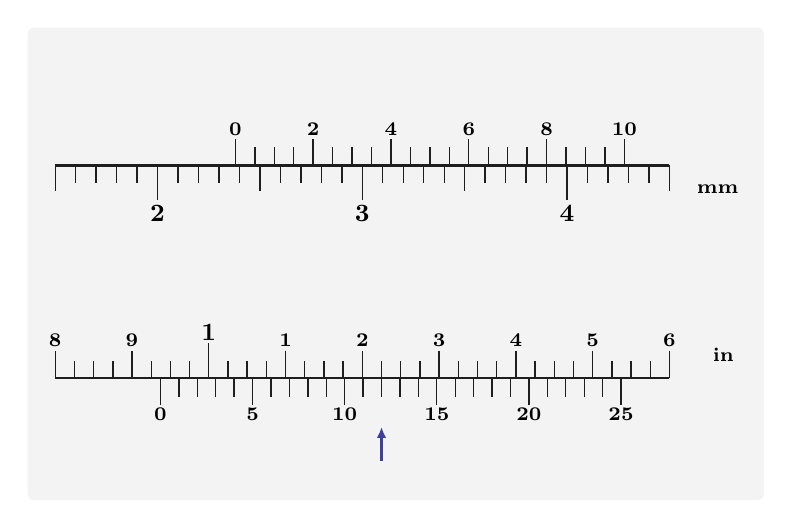
\begin{tikzpicture}[scale=1]
  \fill[figpanel,rounded corners=2pt] (-0.35,-1.55) rectangle (9,4.45);
  \begin{scope}[yshift=2.70cm]
  \draw[scb] (0,0) -- (7.8,0);
  \draw[sc] (0,0) -- (0,-0.32);
  \draw[sc] (0.26,0) -- (0.26,-0.22);
  \draw[sc] (0.52,0) -- (0.52,-0.22);
  \draw[sc] (0.78,0) -- (0.78,-0.22);
  \draw[sc] (1.04,0) -- (1.04,-0.22);
  \draw[sc] (1.3,0) -- (1.3,-0.44);
  \node[lab,below] at (1.3,-0.46) {2};
  \draw[sc] (1.56,0) -- (1.56,-0.22);
  \draw[sc] (1.82,0) -- (1.82,-0.22);
  \draw[sc] (2.08,0) -- (2.08,-0.22);
  \draw[sc] (2.34,0) -- (2.34,-0.22);
  \draw[sc] (2.6,0) -- (2.6,-0.32);
  \draw[sc] (2.86,0) -- (2.86,-0.22);
  \draw[sc] (3.12,0) -- (3.12,-0.22);
  \draw[sc] (3.38,0) -- (3.38,-0.22);
  \draw[sc] (3.64,0) -- (3.64,-0.22);
  \draw[sc] (3.9,0) -- (3.9,-0.44);
  \node[lab,below] at (3.9,-0.46) {3};
  \draw[sc] (4.16,0) -- (4.16,-0.22);
  \draw[sc] (4.42,0) -- (4.42,-0.22);
  \draw[sc] (4.68,0) -- (4.68,-0.22);
  \draw[sc] (4.94,0) -- (4.94,-0.22);
  \draw[sc] (5.2,0) -- (5.2,-0.32);
  \draw[sc] (5.46,0) -- (5.46,-0.22);
  \draw[sc] (5.72,0) -- (5.72,-0.22);
  \draw[sc] (5.98,0) -- (5.98,-0.22);
  \draw[sc] (6.24,0) -- (6.24,-0.22);
  \draw[sc] (6.5,0) -- (6.5,-0.44);
  \node[lab,below] at (6.5,-0.46) {4};
  \draw[sc] (6.76,0) -- (6.76,-0.22);
  \draw[sc] (7.02,0) -- (7.02,-0.22);
  \draw[sc] (7.28,0) -- (7.28,-0.22);
  \draw[sc] (7.54,0) -- (7.54,-0.22);
  \draw[sc] (7.8,0) -- (7.8,-0.32);
  \draw[sc] (2.288,0) -- (2.288,0.34);
  \node[labs,above] at (2.288,0.34) {0};
  \draw[sc] (2.535,0) -- (2.535,0.24);
  \draw[sc] (2.782,0) -- (2.782,0.24);
  \draw[sc] (3.029,0) -- (3.029,0.24);
  \draw[sc] (3.276,0) -- (3.276,0.34);
  \node[labs,above] at (3.276,0.34) {2};
  \draw[sc] (3.523,0) -- (3.523,0.24);
  \draw[sc] (3.77,0) -- (3.77,0.24);
  \draw[sc] (4.017,0) -- (4.017,0.24);
  \draw[sc] (4.264,0) -- (4.264,0.34);
  \node[labs,above] at (4.264,0.34) {4};
  \draw[sc] (4.511,0) -- (4.511,0.24);
  \draw[sc] (4.758,0) -- (4.758,0.24);
  \draw[sc] (5.005,0) -- (5.005,0.24);
  \draw[sc] (5.252,0) -- (5.252,0.34);
  \node[labs,above] at (5.252,0.34) {6};
  \draw[sc] (5.499,0) -- (5.499,0.24);
  \draw[sc] (5.746,0) -- (5.746,0.24);
  \draw[sc] (5.993,0) -- (5.993,0.24);
  \draw[sc] (6.24,0) -- (6.24,0.34);
  \node[labs,above] at (6.24,0.34) {8};
  \draw[sc] (6.487,0) -- (6.487,0.24);
  \draw[sc] (6.734,0) -- (6.734,0.24);
  \draw[sc] (6.981,0) -- (6.981,0.24);
  \draw[sc] (7.228,0) -- (7.228,0.34);
  \node[labs,above] at (7.228,0.34) {10};
  \node[labs,left] at (8.72,-0.30) {mm};
  \end{scope}
  \begin{scope}[yshift=0cm]
  \draw[scb] (0,0) -- (7.8,0);
  \draw[sc] (0,0) -- (0,0.34);
  \node[labs,above] at (0,0.36) {8};
  \draw[sc] (0.2438,0) -- (0.2438,0.22);
  \draw[sc] (0.4875,0) -- (0.4875,0.22);
  \draw[sc] (0.7312,0) -- (0.7312,0.22);
  \draw[sc] (0.975,0) -- (0.975,0.34);
  \node[labs,above] at (0.975,0.36) {9};
  \draw[sc] (1.2188,0) -- (1.2188,0.22);
  \draw[sc] (1.4625,0) -- (1.4625,0.22);
  \draw[sc] (1.7063,0) -- (1.7063,0.22);
  \draw[sc] (1.95,0) -- (1.95,0.44);
  \node[lab,above] at (1.95,0.44) {1};
  \draw[sc] (2.1938,0) -- (2.1938,0.22);
  \draw[sc] (2.4375,0) -- (2.4375,0.22);
  \draw[sc] (2.6812,0) -- (2.6812,0.22);
  \draw[sc] (2.925,0) -- (2.925,0.34);
  \node[labs,above] at (2.925,0.36) {1};
  \draw[sc] (3.1687,0) -- (3.1687,0.22);
  \draw[sc] (3.4125,0) -- (3.4125,0.22);
  \draw[sc] (3.6562,0) -- (3.6562,0.22);
  \draw[sc] (3.9,0) -- (3.9,0.34);
  \node[labs,above] at (3.9,0.36) {2};
  \draw[sc] (4.1438,0) -- (4.1438,0.22);
  \draw[sc] (4.3875,0) -- (4.3875,0.22);
  \draw[sc] (4.6313,0) -- (4.6313,0.22);
  \draw[sc] (4.875,0) -- (4.875,0.34);
  \node[labs,above] at (4.875,0.36) {3};
  \draw[sc] (5.1188,0) -- (5.1188,0.22);
  \draw[sc] (5.3625,0) -- (5.3625,0.22);
  \draw[sc] (5.6062,0) -- (5.6062,0.22);
  \draw[sc] (5.85,0) -- (5.85,0.34);
  \node[labs,above] at (5.85,0.36) {4};
  \draw[sc] (6.0938,0) -- (6.0938,0.22);
  \draw[sc] (6.3375,0) -- (6.3375,0.22);
  \draw[sc] (6.5813,0) -- (6.5813,0.22);
  \draw[sc] (6.825,0) -- (6.825,0.34);
  \node[labs,above] at (6.825,0.36) {5};
  \draw[sc] (7.0688,0) -- (7.0688,0.22);
  \draw[sc] (7.3125,0) -- (7.3125,0.22);
  \draw[sc] (7.5563,0) -- (7.5563,0.22);
  \draw[sc] (7.8,0) -- (7.8,0.34);
  \node[labs,above] at (7.8,0.36) {6};
  \draw[sc] (1.3357,0) -- (1.3357,-0.34);
  \node[labs,below] at (1.3357,-0.34) {0};
  \draw[sc] (1.5698,0) -- (1.5698,-0.24);
  \draw[sc] (1.8038,0) -- (1.8038,-0.24);
  \draw[sc] (2.0378,0) -- (2.0378,-0.24);
  \draw[sc] (2.2718,0) -- (2.2718,-0.24);
  \draw[sc] (2.5057,0) -- (2.5057,-0.34);
  \node[labs,below] at (2.5057,-0.34) {5};
  \draw[sc] (2.7397,0) -- (2.7397,-0.24);
  \draw[sc] (2.9737,0) -- (2.9737,-0.24);
  \draw[sc] (3.2077,0) -- (3.2077,-0.24);
  \draw[sc] (3.4417,0) -- (3.4417,-0.24);
  \draw[sc] (3.6757,0) -- (3.6757,-0.34);
  \node[labs,below] at (3.6757,-0.34) {10};
  \draw[sc] (3.9098,0) -- (3.9098,-0.24);
  \draw[sc] (4.1438,0) -- (4.1438,-0.24);
  \draw[sc] (4.3778,0) -- (4.3778,-0.24);
  \draw[sc] (4.6118,0) -- (4.6118,-0.24);
  \draw[sc] (4.8458,0) -- (4.8458,-0.34);
  \node[labs,below] at (4.8458,-0.34) {15};
  \draw[sc] (5.0798,0) -- (5.0798,-0.24);
  \draw[sc] (5.3138,0) -- (5.3138,-0.24);
  \draw[sc] (5.5477,0) -- (5.5477,-0.24);
  \draw[sc] (5.7817,0) -- (5.7817,-0.24);
  \draw[sc] (6.0157,0) -- (6.0157,-0.34);
  \node[labs,below] at (6.0157,-0.34) {20};
  \draw[sc] (6.2498,0) -- (6.2498,-0.24);
  \draw[sc] (6.4838,0) -- (6.4838,-0.24);
  \draw[sc] (6.7178,0) -- (6.7178,-0.24);
  \draw[sc] (6.9518,0) -- (6.9518,-0.24);
  \draw[sc] (7.1857,0) -- (7.1857,-0.34);
  \node[labs,below] at (7.1857,-0.34) {25};
  \draw[ptr] (4.1438,-1.05) -- (4.1438,-0.62);
  \node[labs,left] at (8.66,0.30) {in};
  \end{scope}
\end{tikzpicture}
}

\newcommand{\figQBC}{%
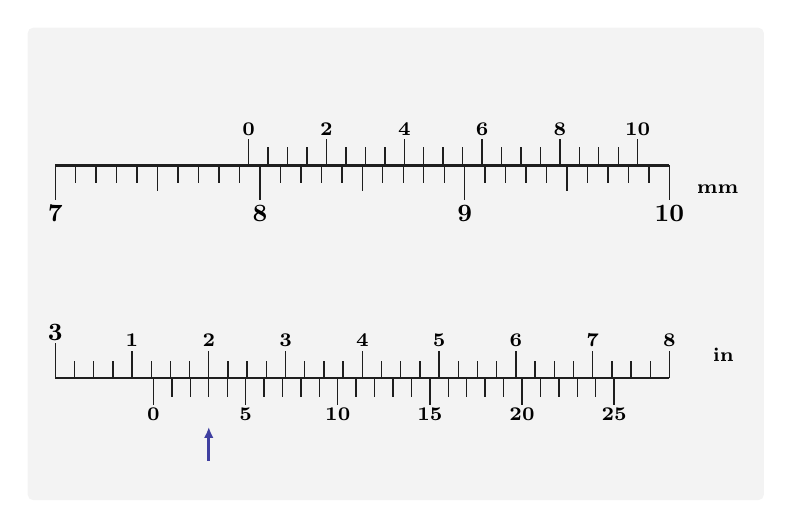
\begin{tikzpicture}[scale=1]
  \fill[figpanel,rounded corners=2pt] (-0.35,-1.55) rectangle (9,4.45);
  \begin{scope}[yshift=2.70cm]
  \draw[scb] (0,0) -- (7.8,0);
  \draw[sc] (0,0) -- (0,-0.44);
  \node[lab,below] at (0,-0.46) {7};
  \draw[sc] (0.26,0) -- (0.26,-0.22);
  \draw[sc] (0.52,0) -- (0.52,-0.22);
  \draw[sc] (0.78,0) -- (0.78,-0.22);
  \draw[sc] (1.04,0) -- (1.04,-0.22);
  \draw[sc] (1.3,0) -- (1.3,-0.32);
  \draw[sc] (1.56,0) -- (1.56,-0.22);
  \draw[sc] (1.82,0) -- (1.82,-0.22);
  \draw[sc] (2.08,0) -- (2.08,-0.22);
  \draw[sc] (2.34,0) -- (2.34,-0.22);
  \draw[sc] (2.6,0) -- (2.6,-0.44);
  \node[lab,below] at (2.6,-0.46) {8};
  \draw[sc] (2.86,0) -- (2.86,-0.22);
  \draw[sc] (3.12,0) -- (3.12,-0.22);
  \draw[sc] (3.38,0) -- (3.38,-0.22);
  \draw[sc] (3.64,0) -- (3.64,-0.22);
  \draw[sc] (3.9,0) -- (3.9,-0.32);
  \draw[sc] (4.16,0) -- (4.16,-0.22);
  \draw[sc] (4.42,0) -- (4.42,-0.22);
  \draw[sc] (4.68,0) -- (4.68,-0.22);
  \draw[sc] (4.94,0) -- (4.94,-0.22);
  \draw[sc] (5.2,0) -- (5.2,-0.44);
  \node[lab,below] at (5.2,-0.46) {9};
  \draw[sc] (5.46,0) -- (5.46,-0.22);
  \draw[sc] (5.72,0) -- (5.72,-0.22);
  \draw[sc] (5.98,0) -- (5.98,-0.22);
  \draw[sc] (6.24,0) -- (6.24,-0.22);
  \draw[sc] (6.5,0) -- (6.5,-0.32);
  \draw[sc] (6.76,0) -- (6.76,-0.22);
  \draw[sc] (7.02,0) -- (7.02,-0.22);
  \draw[sc] (7.28,0) -- (7.28,-0.22);
  \draw[sc] (7.54,0) -- (7.54,-0.22);
  \draw[sc] (7.8,0) -- (7.8,-0.44);
  \node[lab,below] at (7.8,-0.46) {10};
  \draw[sc] (2.457,0) -- (2.457,0.34);
  \node[labs,above] at (2.457,0.34) {0};
  \draw[sc] (2.704,0) -- (2.704,0.24);
  \draw[sc] (2.951,0) -- (2.951,0.24);
  \draw[sc] (3.198,0) -- (3.198,0.24);
  \draw[sc] (3.445,0) -- (3.445,0.34);
  \node[labs,above] at (3.445,0.34) {2};
  \draw[sc] (3.692,0) -- (3.692,0.24);
  \draw[sc] (3.939,0) -- (3.939,0.24);
  \draw[sc] (4.186,0) -- (4.186,0.24);
  \draw[sc] (4.433,0) -- (4.433,0.34);
  \node[labs,above] at (4.433,0.34) {4};
  \draw[sc] (4.68,0) -- (4.68,0.24);
  \draw[sc] (4.927,0) -- (4.927,0.24);
  \draw[sc] (5.174,0) -- (5.174,0.24);
  \draw[sc] (5.421,0) -- (5.421,0.34);
  \node[labs,above] at (5.421,0.34) {6};
  \draw[sc] (5.668,0) -- (5.668,0.24);
  \draw[sc] (5.915,0) -- (5.915,0.24);
  \draw[sc] (6.162,0) -- (6.162,0.24);
  \draw[sc] (6.409,0) -- (6.409,0.34);
  \node[labs,above] at (6.409,0.34) {8};
  \draw[sc] (6.656,0) -- (6.656,0.24);
  \draw[sc] (6.903,0) -- (6.903,0.24);
  \draw[sc] (7.15,0) -- (7.15,0.24);
  \draw[sc] (7.397,0) -- (7.397,0.34);
  \node[labs,above] at (7.397,0.34) {10};
  \node[labs,left] at (8.72,-0.30) {mm};
  \end{scope}
  \begin{scope}[yshift=0cm]
  \draw[scb] (0,0) -- (7.8,0);
  \draw[sc] (0,0) -- (0,0.44);
  \node[lab,above] at (0,0.44) {3};
  \draw[sc] (0.2438,0) -- (0.2438,0.22);
  \draw[sc] (0.4875,0) -- (0.4875,0.22);
  \draw[sc] (0.7313,0) -- (0.7313,0.22);
  \draw[sc] (0.975,0) -- (0.975,0.34);
  \node[labs,above] at (0.975,0.36) {1};
  \draw[sc] (1.2188,0) -- (1.2188,0.22);
  \draw[sc] (1.4625,0) -- (1.4625,0.22);
  \draw[sc] (1.7063,0) -- (1.7063,0.22);
  \draw[sc] (1.95,0) -- (1.95,0.34);
  \node[labs,above] at (1.95,0.36) {2};
  \draw[sc] (2.1938,0) -- (2.1938,0.22);
  \draw[sc] (2.4375,0) -- (2.4375,0.22);
  \draw[sc] (2.6813,0) -- (2.6813,0.22);
  \draw[sc] (2.925,0) -- (2.925,0.34);
  \node[labs,above] at (2.925,0.36) {3};
  \draw[sc] (3.1688,0) -- (3.1688,0.22);
  \draw[sc] (3.4125,0) -- (3.4125,0.22);
  \draw[sc] (3.6562,0) -- (3.6562,0.22);
  \draw[sc] (3.9,0) -- (3.9,0.34);
  \node[labs,above] at (3.9,0.36) {4};
  \draw[sc] (4.1438,0) -- (4.1438,0.22);
  \draw[sc] (4.3875,0) -- (4.3875,0.22);
  \draw[sc] (4.6313,0) -- (4.6313,0.22);
  \draw[sc] (4.875,0) -- (4.875,0.34);
  \node[labs,above] at (4.875,0.36) {5};
  \draw[sc] (5.1188,0) -- (5.1188,0.22);
  \draw[sc] (5.3625,0) -- (5.3625,0.22);
  \draw[sc] (5.6063,0) -- (5.6063,0.22);
  \draw[sc] (5.85,0) -- (5.85,0.34);
  \node[labs,above] at (5.85,0.36) {6};
  \draw[sc] (6.0938,0) -- (6.0938,0.22);
  \draw[sc] (6.3375,0) -- (6.3375,0.22);
  \draw[sc] (6.5813,0) -- (6.5813,0.22);
  \draw[sc] (6.825,0) -- (6.825,0.34);
  \node[labs,above] at (6.825,0.36) {7};
  \draw[sc] (7.0688,0) -- (7.0688,0.22);
  \draw[sc] (7.3125,0) -- (7.3125,0.22);
  \draw[sc] (7.5563,0) -- (7.5563,0.22);
  \draw[sc] (7.8,0) -- (7.8,0.34);
  \node[labs,above] at (7.8,0.36) {8};
  \draw[sc] (1.248,0) -- (1.248,-0.34);
  \node[labs,below] at (1.248,-0.34) {0};
  \draw[sc] (1.482,0) -- (1.482,-0.24);
  \draw[sc] (1.716,0) -- (1.716,-0.24);
  \draw[sc] (1.95,0) -- (1.95,-0.24);
  \draw[sc] (2.184,0) -- (2.184,-0.24);
  \draw[sc] (2.418,0) -- (2.418,-0.34);
  \node[labs,below] at (2.418,-0.34) {5};
  \draw[sc] (2.652,0) -- (2.652,-0.24);
  \draw[sc] (2.886,0) -- (2.886,-0.24);
  \draw[sc] (3.12,0) -- (3.12,-0.24);
  \draw[sc] (3.354,0) -- (3.354,-0.24);
  \draw[sc] (3.588,0) -- (3.588,-0.34);
  \node[labs,below] at (3.588,-0.34) {10};
  \draw[sc] (3.822,0) -- (3.822,-0.24);
  \draw[sc] (4.056,0) -- (4.056,-0.24);
  \draw[sc] (4.29,0) -- (4.29,-0.24);
  \draw[sc] (4.524,0) -- (4.524,-0.24);
  \draw[sc] (4.758,0) -- (4.758,-0.34);
  \node[labs,below] at (4.758,-0.34) {15};
  \draw[sc] (4.992,0) -- (4.992,-0.24);
  \draw[sc] (5.226,0) -- (5.226,-0.24);
  \draw[sc] (5.46,0) -- (5.46,-0.24);
  \draw[sc] (5.694,0) -- (5.694,-0.24);
  \draw[sc] (5.928,0) -- (5.928,-0.34);
  \node[labs,below] at (5.928,-0.34) {20};
  \draw[sc] (6.162,0) -- (6.162,-0.24);
  \draw[sc] (6.396,0) -- (6.396,-0.24);
  \draw[sc] (6.63,0) -- (6.63,-0.24);
  \draw[sc] (6.864,0) -- (6.864,-0.24);
  \draw[sc] (7.098,0) -- (7.098,-0.34);
  \node[labs,below] at (7.098,-0.34) {25};
  \draw[ptr] (1.95,-1.05) -- (1.95,-0.62);
  \node[labs,left] at (8.66,0.30) {in};
  \end{scope}
\end{tikzpicture}
}

\newcommand{\figQBF}{%
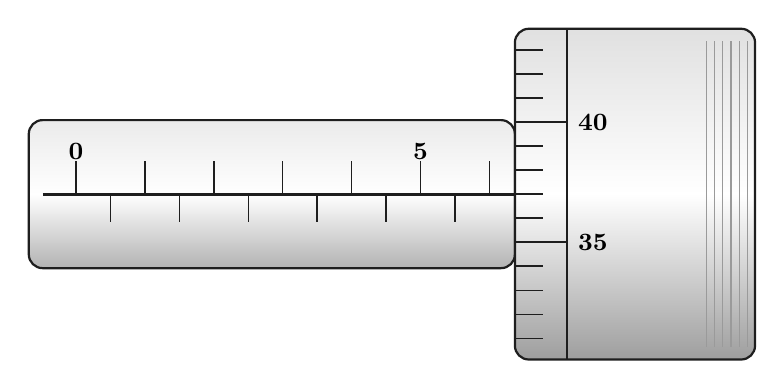
\begin{tikzpicture}[scale=1]
  \shade[rounded corners=5pt,top color=black!8,bottom color=black!30,middle color=white] (0,-0.94) rectangle (6.1738,0.94);
  \draw[scb,rounded corners=5pt] (0,-0.94) rectangle (6.1738,0.94);
  \draw[draw=figline,line width=1.1pt] (0.18,0) -- (6.1738,0);
  \draw[sc] (0.6,0) -- (0.6,0.42);
  \node[lab,above] at (0.6,0.40) {0};
  \draw[sc] (1.0375,0) -- (1.0375,-0.36);
  \draw[sc] (1.475,0) -- (1.475,0.42);
  \draw[sc] (1.9125,0) -- (1.9125,-0.36);
  \draw[sc] (2.35,0) -- (2.35,0.42);
  \draw[sc] (2.7875,0) -- (2.7875,-0.36);
  \draw[sc] (3.225,0) -- (3.225,0.42);
  \draw[sc] (3.6625,0) -- (3.6625,-0.36);
  \draw[sc] (4.1,0) -- (4.1,0.42);
  \draw[sc] (4.5375,0) -- (4.5375,-0.36);
  \draw[sc] (4.975,0) -- (4.975,0.42);
  \node[lab,above] at (4.975,0.40) {5};
  \draw[sc] (5.4125,0) -- (5.4125,-0.36);
  \draw[sc] (5.85,0) -- (5.85,0.42);
  \shade[rounded corners=5pt,top color=black!12,bottom color=black!38,middle color=white] (6.1738,-2.1) rectangle (9.2237,2.1);
  \draw[scb,rounded corners=5pt] (6.1738,-2.1) rectangle (9.2237,2.1);
  \draw[draw=figline,line width=1.0pt] (6.1738,-1.94) -- (6.1738,1.94);
  \draw[sc] (6.8338,-2.1) -- (6.8338,2.1);
  \draw[draw=figline!45,line width=0.4pt] (8.6037,-1.94) -- (8.6037,1.94);
  \draw[draw=figline!45,line width=0.4pt] (8.7088,-1.94) -- (8.7088,1.94);
  \draw[draw=figline!45,line width=0.4pt] (8.8138,-1.94) -- (8.8138,1.94);
  \draw[draw=figline!45,line width=0.4pt] (8.9187,-1.94) -- (8.9187,1.94);
  \draw[draw=figline!45,line width=0.4pt] (9.0237,-1.94) -- (9.0237,1.94);
  \draw[draw=figline!45,line width=0.4pt] (9.1288,-1.94) -- (9.1288,1.94);
  \draw[draw=figline,line width=0.5pt] (6.1738,-1.83) -- (6.5368,-1.83);
  \draw[draw=figline,line width=0.5pt] (6.1738,-1.525) -- (6.5368,-1.525);
  \draw[draw=figline,line width=0.5pt] (6.1738,-1.22) -- (6.5368,-1.22);
  \draw[draw=figline,line width=0.5pt] (6.1738,-0.915) -- (6.5368,-0.915);
  \draw[draw=figline,line width=0.9pt] (6.1738,-0.61) -- (6.8338,-0.61);
  \node[lab,right] at (6.9337,-0.61) {35};
  \draw[draw=figline,line width=0.5pt] (6.1738,-0.305) -- (6.5368,-0.305);
  \draw[draw=figline,line width=0.5pt] (6.1738,0) -- (6.5368,0);
  \draw[draw=figline,line width=0.5pt] (6.1738,0.305) -- (6.5368,0.305);
  \draw[draw=figline,line width=0.5pt] (6.1738,0.61) -- (6.5368,0.61);
  \draw[draw=figline,line width=0.9pt] (6.1738,0.915) -- (6.8338,0.915);
  \node[lab,right] at (6.9337,0.915) {40};
  \draw[draw=figline,line width=0.5pt] (6.1738,1.22) -- (6.5368,1.22);
  \draw[draw=figline,line width=0.5pt] (6.1738,1.525) -- (6.5368,1.525);
  \draw[draw=figline,line width=0.5pt] (6.1738,1.83) -- (6.5368,1.83);
\end{tikzpicture}
}

\newcommand{\figQBG}{%
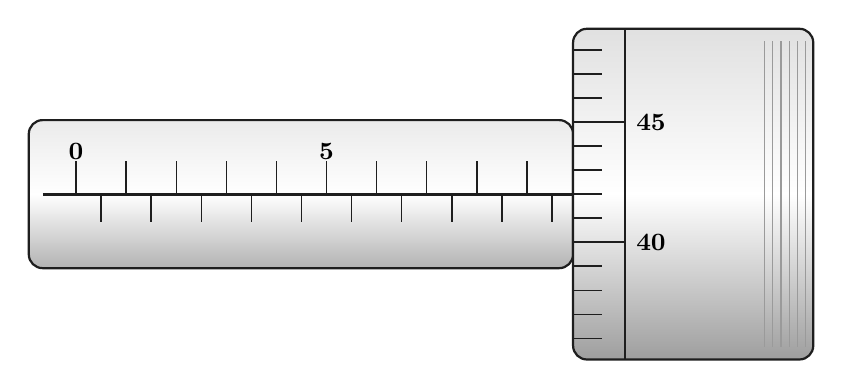
\begin{tikzpicture}[scale=1]
  \shade[rounded corners=5pt,top color=black!8,bottom color=black!30,middle color=white] (0,-0.94) rectangle (6.9127,0.94);
  \draw[scb,rounded corners=5pt] (0,-0.94) rectangle (6.9127,0.94);
  \draw[draw=figline,line width=1.1pt] (0.18,0) -- (6.9127,0);
  \draw[sc] (0.6,0) -- (0.6,0.42);
  \node[lab,above] at (0.6,0.40) {0};
  \draw[sc] (0.9182,0) -- (0.9182,-0.36);
  \draw[sc] (1.2364,0) -- (1.2364,0.42);
  \draw[sc] (1.5545,0) -- (1.5545,-0.36);
  \draw[sc] (1.8727,0) -- (1.8727,0.42);
  \draw[sc] (2.1909,0) -- (2.1909,-0.36);
  \draw[sc] (2.5091,0) -- (2.5091,0.42);
  \draw[sc] (2.8273,0) -- (2.8273,-0.36);
  \draw[sc] (3.1455,0) -- (3.1455,0.42);
  \draw[sc] (3.4636,0) -- (3.4636,-0.36);
  \draw[sc] (3.7818,0) -- (3.7818,0.42);
  \node[lab,above] at (3.7818,0.40) {5};
  \draw[sc] (4.1,0) -- (4.1,-0.36);
  \draw[sc] (4.4182,0) -- (4.4182,0.42);
  \draw[sc] (4.7364,0) -- (4.7364,-0.36);
  \draw[sc] (5.0545,0) -- (5.0545,0.42);
  \draw[sc] (5.3727,0) -- (5.3727,-0.36);
  \draw[sc] (5.6909,0) -- (5.6909,0.42);
  \draw[sc] (6.0091,0) -- (6.0091,-0.36);
  \draw[sc] (6.3273,0) -- (6.3273,0.42);
  \draw[sc] (6.6455,0) -- (6.6455,-0.36);
  \shade[rounded corners=5pt,top color=black!12,bottom color=black!38,middle color=white] (6.9127,-2.1) rectangle (9.9627,2.1);
  \draw[scb,rounded corners=5pt] (6.9127,-2.1) rectangle (9.9627,2.1);
  \draw[draw=figline,line width=1.0pt] (6.9127,-1.94) -- (6.9127,1.94);
  \draw[sc] (7.5727,-2.1) -- (7.5727,2.1);
  \draw[draw=figline!45,line width=0.4pt] (9.3427,-1.94) -- (9.3427,1.94);
  \draw[draw=figline!45,line width=0.4pt] (9.4477,-1.94) -- (9.4477,1.94);
  \draw[draw=figline!45,line width=0.4pt] (9.5527,-1.94) -- (9.5527,1.94);
  \draw[draw=figline!45,line width=0.4pt] (9.6577,-1.94) -- (9.6577,1.94);
  \draw[draw=figline!45,line width=0.4pt] (9.7627,-1.94) -- (9.7627,1.94);
  \draw[draw=figline!45,line width=0.4pt] (9.8677,-1.94) -- (9.8677,1.94);
  \draw[draw=figline,line width=0.5pt] (6.9127,-1.83) -- (7.2757,-1.83);
  \draw[draw=figline,line width=0.5pt] (6.9127,-1.525) -- (7.2757,-1.525);
  \draw[draw=figline,line width=0.5pt] (6.9127,-1.22) -- (7.2757,-1.22);
  \draw[draw=figline,line width=0.5pt] (6.9127,-0.915) -- (7.2757,-0.915);
  \draw[draw=figline,line width=0.9pt] (6.9127,-0.61) -- (7.5727,-0.61);
  \node[lab,right] at (7.6727,-0.61) {40};
  \draw[draw=figline,line width=0.5pt] (6.9127,-0.305) -- (7.2757,-0.305);
  \draw[draw=figline,line width=0.5pt] (6.9127,0) -- (7.2757,0);
  \draw[draw=figline,line width=0.5pt] (6.9127,0.305) -- (7.2757,0.305);
  \draw[draw=figline,line width=0.5pt] (6.9127,0.61) -- (7.2757,0.61);
  \draw[draw=figline,line width=0.9pt] (6.9127,0.915) -- (7.5727,0.915);
  \node[lab,right] at (7.6727,0.915) {45};
  \draw[draw=figline,line width=0.5pt] (6.9127,1.22) -- (7.2757,1.22);
  \draw[draw=figline,line width=0.5pt] (6.9127,1.525) -- (7.2757,1.525);
  \draw[draw=figline,line width=0.5pt] (6.9127,1.83) -- (7.2757,1.83);
\end{tikzpicture}
}

\newcommand{\figQBH}{%
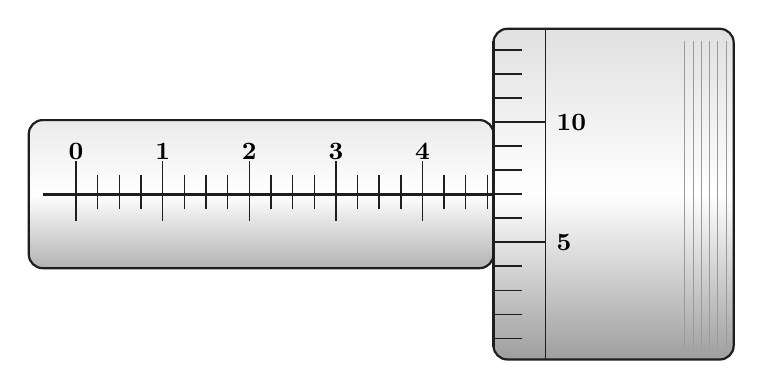
\begin{tikzpicture}[scale=1]
  \shade[rounded corners=5pt,top color=black!8,bottom color=black!30,middle color=white] (0,-0.94) rectangle (5.902,0.94);
  \draw[scb,rounded corners=5pt] (0,-0.94) rectangle (5.902,0.94);
  \draw[draw=figline,line width=1.1pt] (0.18,0) -- (5.902,0);
  \draw[sc] (0.6,-0.336) -- (0.6,0.42);
  \node[lab,above] at (0.6,0.40) {0};
  \draw[sc] (0.875,-0.192) -- (0.875,0.24);
  \draw[sc] (1.15,-0.192) -- (1.15,0.24);
  \draw[sc] (1.425,-0.192) -- (1.425,0.24);
  \draw[sc] (1.7,-0.336) -- (1.7,0.42);
  \node[lab,above] at (1.7,0.40) {1};
  \draw[sc] (1.975,-0.192) -- (1.975,0.24);
  \draw[sc] (2.25,-0.192) -- (2.25,0.24);
  \draw[sc] (2.525,-0.192) -- (2.525,0.24);
  \draw[sc] (2.8,-0.336) -- (2.8,0.42);
  \node[lab,above] at (2.8,0.40) {2};
  \draw[sc] (3.075,-0.192) -- (3.075,0.24);
  \draw[sc] (3.35,-0.192) -- (3.35,0.24);
  \draw[sc] (3.625,-0.192) -- (3.625,0.24);
  \draw[sc] (3.9,-0.336) -- (3.9,0.42);
  \node[lab,above] at (3.9,0.40) {3};
  \draw[sc] (4.175,-0.192) -- (4.175,0.24);
  \draw[sc] (4.45,-0.192) -- (4.45,0.24);
  \draw[sc] (4.725,-0.192) -- (4.725,0.24);
  \draw[sc] (5,-0.336) -- (5,0.42);
  \node[lab,above] at (5,0.40) {4};
  \draw[sc] (5.275,-0.192) -- (5.275,0.24);
  \draw[sc] (5.55,-0.192) -- (5.55,0.24);
  \draw[sc] (5.825,-0.192) -- (5.825,0.24);
  \shade[rounded corners=5pt,top color=black!12,bottom color=black!38,middle color=white] (5.902,-2.1) rectangle (8.952,2.1);
  \draw[scb,rounded corners=5pt] (5.902,-2.1) rectangle (8.952,2.1);
  \draw[draw=figline,line width=1.0pt] (5.902,-1.94) -- (5.902,1.94);
  \draw[sc] (6.562,-2.1) -- (6.562,2.1);
  \draw[draw=figline!45,line width=0.4pt] (8.332,-1.94) -- (8.332,1.94);
  \draw[draw=figline!45,line width=0.4pt] (8.437,-1.94) -- (8.437,1.94);
  \draw[draw=figline!45,line width=0.4pt] (8.542,-1.94) -- (8.542,1.94);
  \draw[draw=figline!45,line width=0.4pt] (8.647,-1.94) -- (8.647,1.94);
  \draw[draw=figline!45,line width=0.4pt] (8.752,-1.94) -- (8.752,1.94);
  \draw[draw=figline!45,line width=0.4pt] (8.857,-1.94) -- (8.857,1.94);
  \draw[draw=figline,line width=0.5pt] (5.902,-1.83) -- (6.265,-1.83);
  \draw[draw=figline,line width=0.5pt] (5.902,-1.525) -- (6.265,-1.525);
  \draw[draw=figline,line width=0.5pt] (5.902,-1.22) -- (6.265,-1.22);
  \draw[draw=figline,line width=0.5pt] (5.902,-0.915) -- (6.265,-0.915);
  \draw[draw=figline,line width=0.9pt] (5.902,-0.61) -- (6.562,-0.61);
  \node[lab,right] at (6.662,-0.61) {5};
  \draw[draw=figline,line width=0.5pt] (5.902,-0.305) -- (6.265,-0.305);
  \draw[draw=figline,line width=0.5pt] (5.902,0) -- (6.265,0);
  \draw[draw=figline,line width=0.5pt] (5.902,0.305) -- (6.265,0.305);
  \draw[draw=figline,line width=0.5pt] (5.902,0.61) -- (6.265,0.61);
  \draw[draw=figline,line width=0.9pt] (5.902,0.915) -- (6.562,0.915);
  \node[lab,right] at (6.662,0.915) {10};
  \draw[draw=figline,line width=0.5pt] (5.902,1.22) -- (6.265,1.22);
  \draw[draw=figline,line width=0.5pt] (5.902,1.525) -- (6.265,1.525);
  \draw[draw=figline,line width=0.5pt] (5.902,1.83) -- (6.265,1.83);
\end{tikzpicture}
}

\newcommand{\figQBI}{%
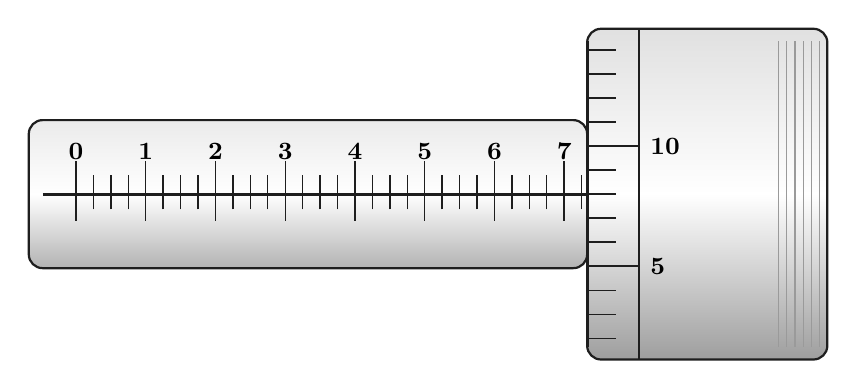
\begin{tikzpicture}[scale=1]
  \shade[rounded corners=5pt,top color=black!8,bottom color=black!30,middle color=white] (0,-0.94) rectangle (7.0915,0.94);
  \draw[scb,rounded corners=5pt] (0,-0.94) rectangle (7.0915,0.94);
  \draw[draw=figline,line width=1.1pt] (0.18,0) -- (7.0915,0);
  \draw[sc] (0.6,-0.336) -- (0.6,0.42);
  \node[lab,above] at (0.6,0.40) {0};
  \draw[sc] (0.8214,-0.192) -- (0.8214,0.24);
  \draw[sc] (1.0428,-0.192) -- (1.0428,0.24);
  \draw[sc] (1.2642,-0.192) -- (1.2642,0.24);
  \draw[sc] (1.4856,-0.336) -- (1.4856,0.42);
  \node[lab,above] at (1.4856,0.40) {1};
  \draw[sc] (1.707,-0.192) -- (1.707,0.24);
  \draw[sc] (1.9284,-0.192) -- (1.9284,0.24);
  \draw[sc] (2.1498,-0.192) -- (2.1498,0.24);
  \draw[sc] (2.3712,-0.336) -- (2.3712,0.42);
  \node[lab,above] at (2.3712,0.40) {2};
  \draw[sc] (2.5926,-0.192) -- (2.5926,0.24);
  \draw[sc] (2.814,-0.192) -- (2.814,0.24);
  \draw[sc] (3.0354,-0.192) -- (3.0354,0.24);
  \draw[sc] (3.2568,-0.336) -- (3.2568,0.42);
  \node[lab,above] at (3.2568,0.40) {3};
  \draw[sc] (3.4782,-0.192) -- (3.4782,0.24);
  \draw[sc] (3.6996,-0.192) -- (3.6996,0.24);
  \draw[sc] (3.921,-0.192) -- (3.921,0.24);
  \draw[sc] (4.1424,-0.336) -- (4.1424,0.42);
  \node[lab,above] at (4.1424,0.40) {4};
  \draw[sc] (4.3638,-0.192) -- (4.3638,0.24);
  \draw[sc] (4.5852,-0.192) -- (4.5852,0.24);
  \draw[sc] (4.8066,-0.192) -- (4.8066,0.24);
  \draw[sc] (5.028,-0.336) -- (5.028,0.42);
  \node[lab,above] at (5.028,0.40) {5};
  \draw[sc] (5.2494,-0.192) -- (5.2494,0.24);
  \draw[sc] (5.4708,-0.192) -- (5.4708,0.24);
  \draw[sc] (5.6923,-0.192) -- (5.6923,0.24);
  \draw[sc] (5.9137,-0.336) -- (5.9137,0.42);
  \node[lab,above] at (5.9137,0.40) {6};
  \draw[sc] (6.1351,-0.192) -- (6.1351,0.24);
  \draw[sc] (6.3565,-0.192) -- (6.3565,0.24);
  \draw[sc] (6.5779,-0.192) -- (6.5779,0.24);
  \draw[sc] (6.7993,-0.336) -- (6.7993,0.42);
  \node[lab,above] at (6.7993,0.40) {7};
  \draw[sc] (7.0207,-0.192) -- (7.0207,0.24);
  \shade[rounded corners=5pt,top color=black!12,bottom color=black!38,middle color=white] (7.0915,-2.1) rectangle (10.1415,2.1);
  \draw[scb,rounded corners=5pt] (7.0915,-2.1) rectangle (10.1415,2.1);
  \draw[draw=figline,line width=1.0pt] (7.0915,-1.94) -- (7.0915,1.94);
  \draw[sc] (7.7515,-2.1) -- (7.7515,2.1);
  \draw[draw=figline!45,line width=0.4pt] (9.5215,-1.94) -- (9.5215,1.94);
  \draw[draw=figline!45,line width=0.4pt] (9.6265,-1.94) -- (9.6265,1.94);
  \draw[draw=figline!45,line width=0.4pt] (9.7315,-1.94) -- (9.7315,1.94);
  \draw[draw=figline!45,line width=0.4pt] (9.8365,-1.94) -- (9.8365,1.94);
  \draw[draw=figline!45,line width=0.4pt] (9.9415,-1.94) -- (9.9415,1.94);
  \draw[draw=figline!45,line width=0.4pt] (10.0465,-1.94) -- (10.0465,1.94);
  \draw[draw=figline,line width=0.5pt] (7.0915,-1.83) -- (7.4545,-1.83);
  \draw[draw=figline,line width=0.5pt] (7.0915,-1.525) -- (7.4545,-1.525);
  \draw[draw=figline,line width=0.5pt] (7.0915,-1.22) -- (7.4545,-1.22);
  \draw[draw=figline,line width=0.9pt] (7.0915,-0.915) -- (7.7515,-0.915);
  \node[lab,right] at (7.8515,-0.915) {5};
  \draw[draw=figline,line width=0.5pt] (7.0915,-0.61) -- (7.4545,-0.61);
  \draw[draw=figline,line width=0.5pt] (7.0915,-0.305) -- (7.4545,-0.305);
  \draw[draw=figline,line width=0.5pt] (7.0915,0) -- (7.4545,0);
  \draw[draw=figline,line width=0.5pt] (7.0915,0.305) -- (7.4545,0.305);
  \draw[draw=figline,line width=0.9pt] (7.0915,0.61) -- (7.7515,0.61);
  \node[lab,right] at (7.8515,0.61) {10};
  \draw[draw=figline,line width=0.5pt] (7.0915,0.915) -- (7.4545,0.915);
  \draw[draw=figline,line width=0.5pt] (7.0915,1.22) -- (7.4545,1.22);
  \draw[draw=figline,line width=0.5pt] (7.0915,1.525) -- (7.4545,1.525);
  \draw[draw=figline,line width=0.5pt] (7.0915,1.83) -- (7.4545,1.83);
\end{tikzpicture}
}


\begin{document}

\begin{center}
  {\LARGE\bfseries EnergyTech}\\[2pt]
  {\Large Chapter 04 --- Version C}\\[6pt]
  Name: \rule{4.5cm}{0.4pt}\quad Group: \rule{3cm}{0.4pt}\quad SPSP ID: \rule{3.5cm}{0.4pt}
\end{center}

\begin{multicols}{2}
\raggedcolumns
% ---------------- Q1 ----------------
\begin{Qbox}{1}{4-1.1}
Determine the accuracy of the measurement; that is, give the number of significant digits for the measurement.\par\medskip $690{,}000$ lb
\begin{choices}
  \item 3
  \item 1
  \item 6
  \item 2
\end{choices}
\qrcode[height=2.2cm,hyperlink]{https://www.youtube.com/watch?v=FhLOHZ4jlP8}
\end{Qbox}

% ---------------- Q2 ----------------
\begin{Qbox}{2}{4-1.1}
Determine the accuracy of the measurement; that is, give the number of significant digits for the measurement.\par\medskip $250{,}7\overline{0}0$
\begin{choices}
  \item 6
  \item 4
  \item 5
  \item 7
\end{choices}
\qrcode[height=2.2cm,hyperlink]{https://www.youtube.com/watch?v=O2WRBUsIeZc}
\end{Qbox}

% ---------------- Q3 ----------------
\begin{Qbox}{3}{4-1.1}
Determine the accuracy of the measurement; that is, give the number of significant digits for the measurement.\par\medskip $0.00700$ g
\begin{choices}
  \item 4
  \item 3
  \item 2
  \item 6
\end{choices}
\qrcode[height=2.2cm,hyperlink]{https://www.youtube.com/watch?v=29VCgAWuS08}
\end{Qbox}

% ---------------- Q4 ----------------
\begin{Qbox}{4}{4-1.1}
Determine the accuracy of the measurement; that is, give the number of significant digits for the measurement.\par\medskip $0.0902000$ A
\begin{choices}
  \item 7
  \item 6
  \item 5
  \item 8
\end{choices}
\qrcode[height=2.2cm,hyperlink]{https://www.youtube.com/watch?v=gEq2wwiqNB8}
\end{Qbox}

% ---------------- Q5 ----------------
\begin{Qbox}{5}{4-1.1}
Determine the accuracy of the measurement; that is, give the number of significant digits for the measurement.\par\medskip $5{,}024$ m
\begin{choices}
  \item 4
  \item 6
  \item 5
  \item 3
\end{choices}
\qrcode[height=2.2cm,hyperlink]{https://www.youtube.com/watch?v=_FD3dS7Vg3U}
\end{Qbox}

% ---------------- Q6 ----------------
\begin{Qbox}{6}{4-1.1}
Determine the accuracy of the measurement; that is, give the number of significant digits for the measurement.\par\medskip $391{,}500$ g
\begin{choices}
  \item 3
  \item 5
  \item 6
  \item 4
\end{choices}
\qrcode[height=2.2cm,hyperlink]{https://www.youtube.com/watch?v=NZMZXixpuv4}
\end{Qbox}

% ---------------- Q7 ----------------
\begin{Qbox}{7}{4-2.1}
The measurement is 5.630 A. Find the precision.
\begin{choices}
  \item The precision of the measurement is 0.0001 A
  \item The precision of the measurement is 0.00001 A
  \item The precision of the measurement is 0.01 A
  \item The precision of the measurement is 0.001 A
\end{choices}
\qrcode[height=2.2cm,hyperlink]{https://www.youtube.com/watch?v=xKxx56lye3g}
\end{Qbox}

% ---------------- Q8 ----------------
\begin{Qbox}{8}{4-2.1}
The measurement is 92.5 cm. Find the precision.
\begin{choices}
  \item The precision is 0.1 cm
  \item The precision is 0.01 cm
  \item The precision is 1 cm
  \item The precision is 0.001 cm
\end{choices}
\qrcode[height=2.2cm,hyperlink]{https://www.youtube.com/watch?v=1JnWFd0IspY}
\end{Qbox}

% ---------------- Q9 ----------------
\begin{Qbox}{9}{4-2.1}
The measurement is 41.00000 in. Find the precision.
\begin{choices}
  \item The precision is 0.0000001 in
  \item The precision is 0.0001 in
  \item The precision is 0.000001 in
  \item The precision is 0.00001 in
\end{choices}
\qrcode[height=2.2cm,hyperlink]{https://www.youtube.com/watch?v=kZ6FfJt_LTA}
\end{Qbox}

% ---------------- Q10 ----------------
\begin{Qbox}{10}{4-2.1}
The measurement is 615 km. Find the precision.
\begin{choices}
  \item The precision is 0.1 km
  \item The precision is 1 km
  \item The precision is 0.01 km
  \item The precision is 10 km
\end{choices}
\qrcode[height=2.2cm,hyperlink]{https://www.youtube.com/watch?v=Uptz7jfWnVI}
\end{Qbox}

% ---------------- Q11 ----------------
\begin{Qbox}{11}{4-2.1}
The measurement is $4{,}\overline{0}00$ mi. Find the precision.
\begin{choices}
  \item The precision is 1000 mi
  \item The precision is 100 mi
  \item The precision is 1 mi
  \item The precision is 10 mi
\end{choices}
\qrcode[height=2.2cm,hyperlink]{https://www.youtube.com/watch?v=SE7YQtbcBeg}
\end{Qbox}

% ---------------- Q12 ----------------
\begin{Qbox}{12}{4-2.1}
The measurement is 8.4090 mi. Find the precision.
\begin{choices}
  \item The precision is 0.000001 mi
  \item The precision is 0.001 mi
  \item The precision is 0.00001 mi
  \item The precision is 0.0001 mi
\end{choices}
\qrcode[height=2.2cm,hyperlink]{https://www.youtube.com/watch?v=cksn4vK3mhk}
\end{Qbox}

% ---------------- Q13 ----------------
\begin{Qbox}{13}{4-2.2}
The measurement is 21.7500 cm. Find the greatest possible error of the measurement.
\begin{choices}
  \item The greatest possible error is 0.0005 cm
  \item The greatest possible error is 0.000005 cm
  \item The greatest possible error is 0.0001 cm
  \item The greatest possible error is 0.00005 cm
\end{choices}
\qrcode[height=2.2cm,hyperlink]{https://www.youtube.com/watch?v=L-TsjdvD7ZQ}
\end{Qbox}

% ---------------- Q14 ----------------
\begin{Qbox}{14}{4-2.2}
The measurement is 6.320 m. Find the greatest possible error of the measurement.
\begin{choices}
  \item The greatest possible error is 0.00005 m
  \item The greatest possible error is 0.001 m
  \item The greatest possible error is 0.0005 m
  \item The greatest possible error is 0.005 m
\end{choices}
\qrcode[height=2.2cm,hyperlink]{https://www.youtube.com/watch?v=QKBMWpAA95s}
\end{Qbox}

% ---------------- Q15 ----------------
\begin{Qbox}{15}{4-2.2}
The measurement is 82.4 m. Find the greatest possible error of the measurement.
\begin{choices}
  \item The greatest possible error is 0.5 m
  \item The greatest possible error is 0.05 m
  \item The greatest possible error is 0.1 m
  \item The greatest possible error is 0.005 m
\end{choices}
\qrcode[height=2.2cm,hyperlink]{https://www.youtube.com/watch?v=7kzsFh5ax-8}
\end{Qbox}

% ---------------- Q16 ----------------
\begin{Qbox}{16}{4-2.1 / 4-2.2}
The measurement is $13\frac{5}{24}$ in. Find the precision and the greatest possible error of the measurement.
\begin{choices}
  \item Precision $=\dfrac{1}{48}$, greatest possible error $=\dfrac{1}{24}$
  \item Precision $=\dfrac{1}{24}$, greatest possible error $=\dfrac{1}{24}$
  \item Precision $=\dfrac{1}{24}$, greatest possible error $=\dfrac{1}{48}$
  \item Precision $=\dfrac{1}{48}$, greatest possible error $=\dfrac{1}{48}$
\end{choices}
\qrcode[height=2.2cm,hyperlink]{https://www.youtube.com/watch?v=FbGULnhUr58}
\end{Qbox}

% ---------------- Q17 ----------------
\begin{Qbox}{17}{4-2.1 / 4-2.2}
The measurement is $9\frac{17}{32}$ in. Find the precision and the greatest possible error of the measurement.
\begin{choices}
  \item Precision $=\dfrac{1}{64}$, greatest possible error $=\dfrac{1}{64}$
  \item Precision $=\dfrac{1}{32}$, greatest possible error $=\dfrac{1}{32}$
  \item Precision $=\dfrac{1}{32}$, greatest possible error $=\dfrac{1}{64}$
  \item Precision $=\dfrac{1}{64}$, greatest possible error $=\dfrac{1}{32}$
\end{choices}
\qrcode[height=2.2cm,hyperlink]{https://www.youtube.com/watch?v=8v8T6GLrV7M}
\end{Qbox}

% ---------------- Q18 ----------------
\begin{Qbox}{18}{4-3.1}
In the given Vernier Caliper, part M is \ldots
\incfig{210}{fig_caliper.png}
\begin{choices}
  \item Depth gauge
  \item Beam
  \item Small jaws
  \item Jaws
\end{choices}
\qrcode[height=2.2cm,hyperlink]{https://www.youtube.com/watch?v=CKAhOUBv_Ck}
\end{Qbox}

% ---------------- Q19 ----------------
\begin{Qbox}{19}{4-3.1}
In the given Vernier Caliper, part L is \ldots
\incfig{210}{fig_caliper.png}
\begin{choices}
  \item Metric Vernier scale
  \item U.S. Fixed scale
  \item Metric Fixed scale
  \item U.S. Vernier scale
\end{choices}
\qrcode[height=2.2cm,hyperlink]{https://www.youtube.com/watch?v=eydw_enMeQk}
\end{Qbox}

% ---------------- Q20 ----------------
\begin{Qbox}{20}{4-3.1}
Read the measurement in millimeter shown on the vernier caliper.
\figbox{\figQBZ}
\begin{choices}
  \item 64.58 mm
  \item 2.553 mm
  \item 2.535 mm
  \item 64.85 mm
\end{choices}
\qrcode[height=2.2cm,hyperlink]{https://www.youtube.com/watch?v=m5Lp71cWcFE}
\end{Qbox}

% ---------------- Q21 ----------------
\begin{Qbox}{21}{4-3.2}
Read the measurement in millimeter shown on the vernier caliper.
\figbox{\figQBA}
\begin{choices}
  \item 128.02 mm
  \item 5.074 mm
  \item 5.047 mm
  \item 128.20 mm
\end{choices}
\qrcode[height=2.2cm,hyperlink]{https://www.youtube.com/watch?v=xVg0hxrQ4Jg}
\end{Qbox}

% ---------------- Q22 ----------------
\begin{Qbox}{22}{4-3.3}
Read the measurement in inch shown on the vernier caliper.
\figbox{\figQBB}
\begin{choices}
  \item 9.370 in
  \item 0.973 in
  \item 23.80 in
  \item 0.937 in
\end{choices}
\qrcode[height=2.2cm,hyperlink]{https://www.youtube.com/watch?v=wcmLZgkqi3M}
\end{Qbox}

% ---------------- Q23 ----------------
\begin{Qbox}{23}{4-3.3}
Read the measurement in inch shown on the vernier caliper.
\figbox{\figQBC}
\begin{choices}
  \item 3.128 in
  \item 3.182 in
  \item 0.128 in
  \item 79.45 in
\end{choices}
\qrcode[height=2.2cm,hyperlink]{https://www.youtube.com/watch?v=bXo3POT01eE}
\end{Qbox}

% ---------------- Q24 ----------------
\begin{Qbox}{24}{4-4.1}
In the given Micrometer Caliper, part F is
\incfig{200}{fig_micrometer.png}
\begin{choices}
  \item Spindle
  \item Anvil
  \item Thimble
  \item Ratchet
\end{choices}
\qrcode[height=2.2cm,hyperlink]{https://www.youtube.com/watch?v=0XkBVkZvfvA}
\end{Qbox}

% ---------------- Q25 ----------------
\begin{Qbox}{25}{4-4.1}
In the given Micrometer Caliper, part K is
\incfig{200}{fig_micrometer.png}
\begin{choices}
  \item Ratchet
  \item Thimble
  \item Anvil
  \item Spindle
\end{choices}
\qrcode[height=2.2cm,hyperlink]{https://www.youtube.com/watch?v=89Bz6HZpME8}
\end{Qbox}

% ---------------- Q26 ----------------
\begin{Qbox}{26}{4-4.2}
Read the measurement shown on the metric micrometer.
\figbox{\figQBF}
\begin{choices}
  \item 6.36 mm
  \item 6.38 mm
  \item 63.7 mm
  \item 6.37 mm
\end{choices}
\qrcode[height=2.2cm,hyperlink]{https://www.youtube.com/watch?v=n0lpdXKX8NA}
\end{Qbox}

% ---------------- Q27 ----------------
\begin{Qbox}{27}{4-4.2}
Read the measurement shown on the metric micrometer.
\figbox{\figQBG}
\begin{choices}
  \item 9.92 mm
  \item 9.93 mm
  \item 99.2 mm
  \item 9.42 mm
\end{choices}
\qrcode[height=2.2cm,hyperlink]{https://www.youtube.com/watch?v=MplthM6FZQU}
\end{Qbox}

% ---------------- Q28 ----------------
\begin{Qbox}{28}{4-4.4}
Read the measurement shown on the U.S. micrometer.
\figbox{\figQBH}
\begin{choices}
  \item 0.482 in
  \item 0.475 in
  \item 0.507 in
  \item 4.820 in
\end{choices}
\qrcode[height=2.2cm,hyperlink]{https://www.youtube.com/watch?v=tTfhEPs7AG4}
\end{Qbox}

% ---------------- Q29 ----------------
\begin{Qbox}{29}{4-4.3}
Read the measurement shown on the U.S. micrometer.
\figbox{\figQBI}
\begin{choices}
  \item 0.725 in
  \item 0.758 in
  \item 0.733 in
  \item 7.330 in
\end{choices}
\qrcode[height=2.2cm,hyperlink]{https://www.youtube.com/watch?v=BSleiTcnV88}
\end{Qbox}

% ---------------- Q30 ----------------
\begin{Qbox}{30}{4-5.1}
Find the measurement that is the most accurate.
\begin{choices}
  \item 318 ft
  \item 760 ft
  \item 200 ft
  \item 5,400 ft
\end{choices}
\qrcode[height=2.2cm,hyperlink]{https://www.youtube.com/watch?v=wFtUtuKgrnI}
\end{Qbox}

% ---------------- Q31 ----------------
\begin{Qbox}{31}{4-5.1}
Find the measurement that is the most accurate.
\begin{choices}
  \item 350 ft
  \item 627 ft
  \item 800 ft
  \item 2,300 ft
\end{choices}
\qrcode[height=2.2cm,hyperlink]{https://www.youtube.com/watch?v=fi2FP7z8XXk}
\end{Qbox}

% ---------------- Q32 ----------------
\begin{Qbox}{32}{4-5.1}
Find the measurement that is the most accurate.
\begin{choices}
  \item 700 ft
  \item 260 ft
  \item 594 ft
  \item 4,100 ft
\end{choices}
\qrcode[height=2.2cm,hyperlink]{https://www.youtube.com/watch?v=S8T8OfIpWdU}
\end{Qbox}

% ---------------- Q33 ----------------
\begin{Qbox}{33}{4-5.1}
Find the measurement that is the most accurate.
\begin{choices}
  \item 1900 ft
  \item 0.00720 ft
  \item 0.4500 ft
  \item 6000 ft
\end{choices}
\qrcode[height=2.2cm,hyperlink]{https://www.youtube.com/watch?v=kmIhRWkySiY}
\end{Qbox}

% ---------------- Q34 ----------------
\begin{Qbox}{34}{4-5.1}
Find the measurement that is the least accurate.
\begin{choices}
  \item 0.000480 in
  \item 7000 in
  \item 0.00090 in
  \item 36.2000 in
\end{choices}
\qrcode[height=2.2cm,hyperlink]{https://www.youtube.com/watch?v=i50ZER16Vic}
\end{Qbox}

% ---------------- Q35 ----------------
\begin{Qbox}{35}{4-5.1}
Find the measurement that is the least accurate.
\begin{choices}
  \item 25800 m
  \item 340000 m
  \item 1870000 m
  \item 0.00610 m
\end{choices}
\qrcode[height=2.2cm,hyperlink]{https://www.youtube.com/watch?v=M7AB8u72_8k}
\end{Qbox}

% ---------------- Q36 ----------------
\begin{Qbox}{36}{4-5.1}
Find the measurement that is the least accurate.
\begin{choices}
  \item 0.000910 in
  \item 67000 in
  \item 84.0000 in
  \item 5000 in
\end{choices}
\qrcode[height=2.2cm,hyperlink]{https://www.youtube.com/watch?v=d32PX6zaUhM}
\end{Qbox}

% ---------------- Q37 ----------------
\begin{Qbox}{37}{4-5.1}
Find the measurement that is the most accurate.
\begin{choices}
  \item 0.00080 A
  \item 0.0470 A
  \item 0.056 A
  \item 0.057 A
\end{choices}
\qrcode[height=2.2cm,hyperlink]{https://www.youtube.com/watch?v=kfDJ24QBcuI}
\end{Qbox}

% ---------------- Q38 ----------------
\begin{Qbox}{38}{4-5.1}
Find the measurement that is the least accurate.
\begin{choices}
  \item 18,000 V
  \item 73,000 V
  \item 90,000 V
  \item 5,200,000 V
\end{choices}
\qrcode[height=2.2cm,hyperlink]{https://www.youtube.com/watch?v=CdvPb7S0h9Y}
\end{Qbox}

% ---------------- Q39 ----------------
\begin{Qbox}{39}{4-5.1}
Find the measurement that is the least accurate.
\begin{choices}
  \item 7,300 V
  \item 50,000 V
  \item 2,900,000 V
  \item 64,000 V
\end{choices}
\qrcode[height=2.2cm,hyperlink]{https://www.youtube.com/watch?v=mdd_74Yj1iA}
\end{Qbox}

% ---------------- Q40 ----------------
\begin{Qbox}{40}{4-5.1}
Find the measurement that is the least accurate.
\begin{choices}
  \item 78.00 V
  \item 0.0081 V
  \item 0.00450 V
  \item 34,700 V
\end{choices}
\qrcode[height=2.2cm,hyperlink]{https://www.youtube.com/watch?v=L0pMHrjqsEg}
\end{Qbox}

% ---------------- Q41 ----------------
\begin{Qbox}{41}{4-5.1}
Find the measurement that is the least accurate.
\begin{choices}
  \item 9.160 ft
  \item 0.4800 ft
  \item 8.40000 ft
  \item 27,000 ft
\end{choices}
\qrcode[height=2.2cm,hyperlink]{https://www.youtube.com/watch?v=nQ0DitEi1Ps}
\end{Qbox}

% ---------------- Q42 ----------------
\begin{Qbox}{42}{4-5.1}
Find the measurement that is the least accurate.
\begin{choices}
  \item 748 ft
  \item 500 ft
  \item 903 ft
  \item 660 ft
\end{choices}
\qrcode[height=2.2cm,hyperlink]{https://www.youtube.com/watch?v=Y1cHxGjrkjU}
\end{Qbox}

% ---------------- Q43 ----------------
\begin{Qbox}{43}{4-5.1}
Find the measurement that is the least accurate.
\begin{choices}
  \item 574 ft
  \item 800 ft
  \item 631 ft
  \item 490 ft
\end{choices}
\qrcode[height=2.2cm,hyperlink]{https://www.youtube.com/watch?v=eBSkNlhA6Wc}
\end{Qbox}

% ---------------- Q44 ----------------
\begin{Qbox}{44}{4-5.1}
Find the measurement that is the least accurate.
\begin{choices}
  \item 840 ft
  \item 703 ft
  \item 729 ft
  \item 600 ft
\end{choices}
\qrcode[height=2.2cm,hyperlink]{https://www.youtube.com/watch?v=toC9PYl0yHk}
\end{Qbox}

% ---------------- Q45 ----------------
\begin{Qbox}{45}{4-5.1}
Use the rules of measurements to evaluate.\par\medskip $(6{,}700\ \text{cm})(18.00\ \text{cm})$
\begin{choices}
  \item 120,000 cm$^2$
  \item 121,000 cm$^2$
  \item 120,600 cm$^2$
  \item 100,000 cm$^2$
\end{choices}
\qrcode[height=2.2cm,hyperlink]{https://www.youtube.com/watch?v=_Xjo5E_pcYo}
\end{Qbox}

% ---------------- Q46 ----------------
\begin{Qbox}{46}{4-6.1}
Use the rules of measurements to evaluate.\par\medskip $(1{,}800\ \text{m})(90\ \text{m})(2140\ \text{m})$
\begin{choices}
  \item 300,000,000 m$^3$
  \item 346,700,000 m$^3$
  \item 347,000,000 m$^3$
  \item 350,000,000 m$^3$
\end{choices}
\qrcode[height=2.2cm,hyperlink]{https://www.youtube.com/watch?v=vd7Sg-5mZc0}
\end{Qbox}

% ---------------- Q47 ----------------
\begin{Qbox}{47}{4-6.1}
Use the rules of measurements to evaluate.\par\medskip $38{,}400$ V $\div\ 5.6$ A
\begin{choices}
  \item 6,860 V/A
  \item 6,857.1 V/A
  \item 7,000 V/A
  \item 6,900 V/A
\end{choices}
\qrcode[height=2.2cm,hyperlink]{https://www.youtube.com/watch?v=rLAH-4JSDRo}
\end{Qbox}

% ---------------- Q48 ----------------
\begin{Qbox}{48}{4-6.1}
Use the rules of measurements to evaluate.\[ \frac{(2760\ m)(4.5\ L)}{5.0\ s} \]
\begin{choices}
  \item $2{,}484\ mL/s$
  \item $2.500\ mL/s$
  \item $2{,}000\ mL/s$
  \item $2{,}500\ mL/s$
\end{choices}
\qrcode[height=2.2cm,hyperlink]{https://www.youtube.com/watch?v=rGtejzjn64U}
\end{Qbox}

% ---------------- Q49 ----------------
\begin{Qbox}{49}{4-6.1}
Find the area of a rectangle 5.20 cm by 24.0 cm. $(A=l\cdot w)$ (Use the rules for working with measurements).
\begin{choices}
  \item 125 cm$^2$
  \item 100 cm$^2$
  \item 124.8 cm$^2$
  \item 120 cm$^2$
\end{choices}
\qrcode[height=2.2cm,hyperlink]{https://www.youtube.com/watch?v=OVOHkqfkrEI}
\end{Qbox}

% ---------------- Q50 ----------------
\begin{Qbox}{50}{4-6.1}
Find the volume of a rectangular solid when $l=4.60$ ft, $w=9.0$ ft, and $h=27.30$ ft.\par\medskip $V=lwh$, where $l$ length, $w$ width, and $h$ height.\par\medskip (Use the rules for working with measurements)
\begin{choices}
  \item 1,000 ft$^3$
  \item 1,130.22 ft$^3$
  \item 1,130 ft$^3$
  \item 1,100 ft$^3$
\end{choices}
\qrcode[height=2.2cm,hyperlink]{https://www.youtube.com/watch?v=6P8cDZvSm3M}
\end{Qbox}

\end{multicols}
\end{document}
